%\chapter{Úvod}
	\chapter{Introduction}
	
	\section{Motivation}
	\subsection{Motivation for Navigation System}
	Blind and other visually impaired want to be self-sufficient. A possibility to walk from one place in the city to another seems very common to us, but is very challenging for the blinds. They can't go just somewhere without previous preparation. They have to study the area on the maps and try to remember it.
	
	A navigation system can spare them all these time-consuming preparations and give them the required information just in time, when they need them. The trouble is the current systems for navigation of a pedestrian with the sight, just shows his position on the map. A user determines his position by looking around him and comparing it with the situation drawn on map. On the other hand the blinds are not able to do something like this, so they need the system
	helps them even with the process of determining the exact position. 
	
	There are some systems specially designed for blind pedestrians. They can be downloaded from the Apples's App Store or Google's Google Play. Still these systems doesn't provide the user with any info about pedestrian crossings and sidewalks.
	
	\subsection{Motivation for Dialog Systems}
	We, humans, are very good at talking. We talk to each other. So the idea of controlling the software just by talking seems very easy. It would reduce a lot of cognitive overload caused by the user interface. The regular interface for blind have to read aloud the content and how to use it \uv{Send, button, double tap to activate} and \uv{Address, Text field, double tap to edit}. So be able just to talk would reduce the amount of spoken text and reduce the cognitive load.
	
	
	\section{Problem Description}
	The current GPS navigations for sighted person shows only information sufficient to sighted people. It shows only approximate position and just which streets the person should go. A sighted person can look around and find a pedestrian crossing to cross the street. As well the person receive feedback by looking what is drawn on the map and comparing it with what he or she sees around. See fig \ref{fig:sighted-person}.
	
	\begin{figure}[h]
		\centering
		\begin{subfigure}{.5\textwidth}
			\centering
			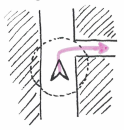
\includegraphics[width=.4\linewidth]{figures/introduction/gps-shows}
			\caption{GPS shows}
			\label{fig:sighted-person-sub1}
		\end{subfigure}%
		\begin{subfigure}{.5\textwidth}
			\centering
			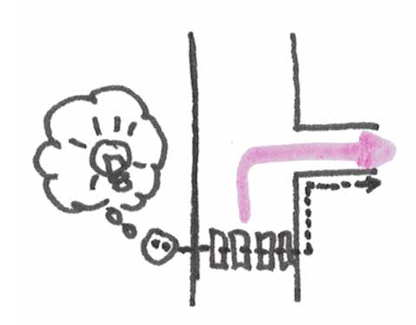
\includegraphics[width=.4\linewidth]{figures/introduction/sighted-person}
			\caption{sighted person analyses}
			\label{fig:sighted-person-sub2}
		\end{subfigure}
		\caption{Info shown by GPS and how a sighted person analyses it}
		\label{fig:sighted-person}
	\end{figure}
	
	On the other hand the blinds can't look around and will not know on which sidewalk they are. And neither the device will know where they exactly are. See fig \ref{fig:blind-person}.
	\begin{figure}[h]
		\centering
		\begin{subfigure}{.5\textwidth}
			\centering
			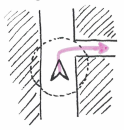
\includegraphics[width=.4\linewidth]{figures/introduction/gps-shows}
			\caption{A subfigure}
			\label{fig:blind-person-sub1}
		\end{subfigure}%
		\begin{subfigure}{.5\textwidth}
			\centering
			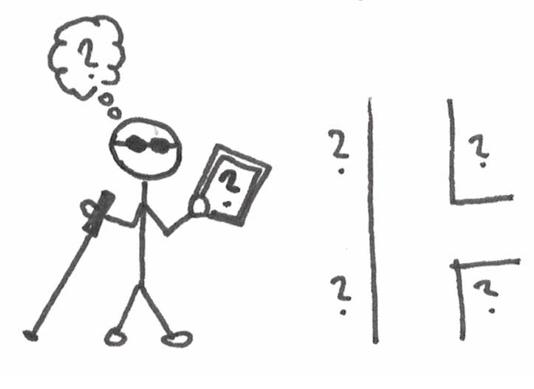
\includegraphics[width=.4\linewidth]{figures/introduction/blind-person}
			\caption{A subfigure}
			\label{fig:blind-person-sub2}
		\end{subfigure}
		\caption{Info shown by GPS and how a sighted person analyses it}
		\label{fig:blind-person}
	\end{figure}
	
	There is a navigation Naviterier in the beta stage of developement. Naviterier can navigate in the manner \uv{cross the pedestrian crossing, turn left, go to corner of a building and turn right}. However Naviterier in the current stage can navigate only from a given Address point to another Address point. I.e. can navigate from \uv{Karlovo náměstí 13} to \uv{Myslíkova 1} (both are streets in Prague, Czech Republic). 
	
	Imagine you have to enter your exact address every time you go somewhere. It is not very convenient. Not talking about cases when you don't know the exact address. i.e. You are on the stop of public transport, you are in the park, someone brought you to a place and now you have to go home. Or you just get lost.
	
	The GPS signal is not sufficiently accurate in the city to estimate the exact position on the sidewalk. The question is can we design a system which using a the inaccurate info from GPS and asking the user some questions can estimate the exact location?
	 
\begin{figure}[h]
	\centering
	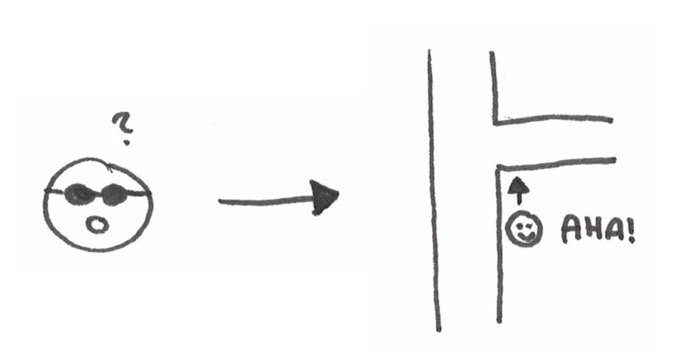
\includegraphics[width=0.7\linewidth]{figures/introduction/determine-exact-position-on-sidewalk}
	\caption[Determine exact position on a sidewalk]{Determine exact position on a sidewalk}
	\label{fig:determine-exact-position-on-sidewalk}
\end{figure}
	
	
	
\begin{figure}[h]
	\centering
	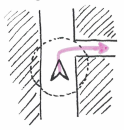
\includegraphics[width=5cm]{figures/introduction/gps-shows}
	\caption[Current Navigations]{Popiska obrázku}
	\label{fig:gps-shows}
\end{figure}

	
	

	
	
	
	
	\section{Expected Goals}
	
	I want to use a dialog system to locate a blind pedestrian.
	
	Popis řešeného problému, vymezení cílů DP/BP a požadavků na implementovaný systém.
	
	
	%*****************************************************************************
	%\chapter{Popis problému, specifikace cíle}
	\chapter{Structure}
	
	Popis struktury DP/BP ve vztahu k vytyčeným cílům.